\documentclass{article}
\usepackage{xcolor}
\usepackage{amsmath}
\usepackage{amssymb}
\usepackage{unicode-math}
\usepackage{makecell}
\usepackage{tabularray}
\usepackage{indentfirst}
\usepackage{booktabs}
\usepackage{amsthm}
\usepackage[hidelinks]{hyperref}
\usepackage{multirow}
\usepackage{pgfplots}
\pgfplotsset{compat=1.18}
\usepackage[style=authoryear, backend=bibtex]{biblatex}
\addbibresource{references.bib}
\usepackage{graphicx} % Required for inserting images
\usepackage[margin=1in]{geometry}
\usepackage{mathtools}

\newcommand{\determinant}[1]{\begin{vmatrix} #1 \end{vmatrix}}

\title{Probability and Statistics - Project 2}
\author{James Keys, Samuel Paez}
\date{April 28, 2026}

\begin{document}

\maketitle

\section{Introduction}\label{sec:introduction}
Statistics, the branch of mathematics that deals with collecting and analyzing real-world data, is of great importance for both prospective and retrospective studies.
In contrast to probability, statistics serves as empirical proof for underlying assumptions people make in their daily lives, suggesting correlation and sometimes even causation.
In this paper, the powerful tools of this field formally introduced in the 17th century will be explored in the context of an intriguing question: do men prefer to marry women that are shorter than them, and does this relate to historical time periods?

\section{Main Goal}\label{sec:main-goal}
In order to aid with the search to a viable answer to this question, the data sets collected by Galton, F. in 1886 and Marsh, C. in 1988 will be utilized, where the heights of couples are provided in inches and millimeters, respectively (Galton's data was converted to mm with the conversion 25.4 mm = 1 inch).
In doing so, we must account for sampling error, the concept that these datasets, despite gathering significant information, may not accurately represent the statistical characteristics of the entire human population.
Furthermore, this project makes use of the \textit{Central Limit Theorem (CLT)}, which states that as the sample size $S$ (the amount of data collected for a particular random variable) increases, the data set distribution will become normal so that
\begin{equation}
p(s)=\frac{e^{-\frac{(s-\mu)^2}{2\sigma^2}}}{\sigma\sqrt{2\pi}}
\label{eq:normal-distribution}
\end{equation}
where $\mu$ is the mean, $\sigma$ is the variance, and $s \in S$.
This iconic theorem also implies that the statistical properties of the sample will approach those of the population so that
\begin{equation}
    \lim_{n\to\infty}\mu_n=\mu
    \qquad\text{and}\qquad
    \lim_{n\to\infty}\sigma_n=\sigma.
    \label{eq:limits-for-central-limit}
\end{equation}

More generally, a random variable is any one-to-one function $V:S\rightarrow{\mathbb{R}}$ that has a discrete or continuous range $R(V)$; these outputs will be denoted as the lowercase version of its random variable.
The following concepts will prove useful as we embark on this endeavor:
\begin{enumerate}
    \item statistic: a value describing the presented data
    \item  hypothesis: a claim about a statistic pertaining to a data set
    \item null hypothesis ($H_0$): a claim that the statistic equals a particular value
    \item alternate hypothesis ($H_a$): a claim that the statistic is not equal to a value and instead is greater or less than it
    \item confidence level: probability that the outcome of a test was not a result of chance
\end{enumerate}

\section{Solution}\label{sec:solution}
\subsection{Part 1:}\label{subsec:part-1:}

% question one is for the mean.
We may begin our analysis by determining some basic facts about our datasets.
We will first calculate the sample mean and standard deviation.
The sample mean is defined as
\begin{equation}
    \overline{x}_n\coloneqq\frac{1}{n}\left(\sum_{k=1}^{n}x_k\right)=\frac{x_1+x_2+\cdots+x_n}{n}
    \label{eq:sample-mean}
\end{equation}

and acts as a simple, unweighted average of the dataset.
The standard deviation is a measure of the amount of variation of a dataset about the average.
It is defined as
\begin{equation}
    \sigma_n\coloneqq\sqrt{\frac{1}{n-1}\sum_{k=1}^n(x_k-\overline{x}_n)^2}.
    \label{eq:sample-std-dev}
\end{equation}
The sample standard deviation includes the $\frac{1}{n-1}$ instead of $\frac{1}{n}$ because the formula which uses the latter fraction is only valid if our sample represents the \textit{entire} population.
Including the $n-1$ term gives the proper unbiased estimator of a larger population.

Tables~\ref{tab:mean-heights} and~\ref{tab:std-heights} present the mean and standard deviation of heights for each sex across both datasets.

\begin{table}[h]
    \centering
    \begin{tabular}{c|cc}
         & Male & Female \\
         \midrule
        Marsh & 1732.4925 & 1601.9497 \\
        Galton & 1760.6289 & 1625.6496 \\
    \end{tabular}
    \caption{Mean heights by sex for each dataset, in mm}
    \label{tab:mean-heights}
\end{table}

\begin{table}[h]
    \centering
    \begin{tabular}{c|cc}
         & Male & Female \\
         \midrule
        Marsh & 68.7507 & 62.4350 \\
        Galton & 67.2387 & 59.2590 \\
    \end{tabular}
    \caption{Standard deviation of heights by sex for each dataset, in mm}
    \label{tab:std-heights}
\end{table}

From Table~\ref{tab:mean-heights}, we can see that men tend to be taller than women on average.
The Marsh dataset also has shorter people on average for both sexes than the Galton dataset.
From these basic observations, we could say that it would not necessarily be surprising for a randomly selected man to be taller than a randomly selected woman.
In addition, the males for both datasets have larger standard deviations in their heights compared to women.

To be able to apply the Central Limit Theorem to this dataset, it is now proper to discuss a joint distribution function that can describe men and women.
This will be useful determining whether these random variables are independent and proving whether there is a relationship between them.
For this purpose, let $Z_1$ and $Z_2$ be two independent random variables, each having a standard normal distribution.
Furthermore, for constants $\mu_1$, $\mu_2$, $\sigma_1$, $\sigma_2$ and $\rho$ such that $-\infty < \mu_i < \infty$, $\sigma_i > 0$ for, $i=1,2$ and $-1 \le \rho \le 1$ we define the following random variables:
\begin{equation}
    X_1 \coloneqq \sigma_1 Z_1 + \mu_1 \qquad X_2 \coloneqq \sigma_2 [\rho Z_1 + (1-\rho^2)^{1/2} Z_2] + \mu_2.
    \label{eq:definitions-of-x-variables}
\end{equation}
To derive the joint density function of these two variables $X_1$ and $X_2$, we can determine the joint density for $Z_1$ and $Z_2$, determine the Jacobian relating the $Z$ variables to the $X$ variables, and then simplify the new equation.
Since $Z_1$ and $Z_2$ are independent, their joint distribution is simply the product of their marginals:
\begin{equation}
    g(z_1, z_2) = g_{Z_1}(z_1)g_{Z_2}(z_2).
    \label{eq:joint-dist-for-independent-vars}
\end{equation}
$Z_1$ and $Z_2$ both have a standard normal distribution, so their individual distribution functions are both of the form:
\begin{equation}
    g_{Z_i}(z_i)=\frac{1}{\sqrt{2\pi}}e^{-\frac{z_i^2}{2}}.
    \label{eq:std-normal-distribution}
\end{equation}
Therefore, the joint distribution for these two variables is
\begin{equation}
    g(z_1,z_2)=\frac{1}{2\pi}\exp\left[-\frac{1}{2}(z_1^2+z_2^2)\right].
    \label{eq:joint-normal-distribution}
\end{equation}
Using a change of variables to translate the probability of a given event from the sample space $Z\in\mathbb{R}^2$ to $X\in\mathbb{R}^2$, the joint density function $f(x_1, x_2)$ will follow this equation:
\begin{equation}
   P = \int_{Z} g(z_1,z_2)dz_2 dz_1= \int_{X} g(\frac{x_1-\mu_1}{\sigma_1},\frac{1}{\sqrt{1-\rho^2}}(\frac{x_2-\mu_2}{\sigma_2}-\rho\frac{x_1-\mu_1}{\sigma_1}))\cdot|J_{\vec{f}}|dz_2 dz_1
    \label{eq:change_of_variables_formula}
\end{equation}
where $J_{\vec{f}}$ is the Jacobian determinant, acknowledging that 
\begin{equation}
    Z_1=\frac{X_1-\mu_1}{\sigma_1} \qquad
    \text{and}\qquad
    Z_2=\frac{1}{\sqrt{1-\rho^2}}\left(\frac{X_2-\mu_2}{\sigma_2}-\rho \left(\frac{X_1-\mu_1}{\sigma_1}\right)\right)
    \label{eq:z-vars-in-x-terms}
\end{equation}
according to \eqref{eq:definitions-of-x-variables}.

To further reduce this expression, it is necessary to define the coordinate transformation vector $\vec{f}\coloneqq\begin{pmatrix}z_1\\z_2\end{pmatrix}$ and find its Jacobian:
\begin{equation}
    J_{\vec{f}}(x_1,x_2)=
    \determinant{
        \frac{\partial}{\partial x_1}z_1 & \frac{\partial}{\partial{x_2}}z_1\\ \frac{\partial}{\partial{x_1}}z_2 & \frac{\partial}{\partial{x_2}}{z_2}
    }=
    \determinant{
        \frac{1}{\sigma} & 0 \\
        \frac{-\rho}{\sigma_1\sqrt{1-\rho^2}} & \frac{1}{\sigma_2\sqrt{1-\rho^2}}
    }
    =\frac{1}{\sigma_1\sigma_2\sqrt{1-\rho^2}}.
    \label{eq:jacobian-determinant.}
\end{equation}
Now, observing that $f(x_1,x_2)=g(z_1,z_2)\cdot J_{\vec{f}}(x_1,x_2) $ we can plug in everything and simplify to introduce what will be referred to as the bivariate normal distribution:
\small
\begin{align*}
    f(x_1,x_2)&=\frac{1}{2\pi\sigma_1\sigma_2\sqrt{1-\rho^2}}
    \exp\left[
        -\frac{1}{2} \left(
            \left( \frac{x_1-\mu_1}{\sigma_1} \right)^2
            +
             \frac{1}{{1-\rho^2}}\left( \frac{x_2-\mu_2}{\sigma_2}-\frac{\rho(x_1-\mu_1)}{\sigma_1} \right)^2
        \right) 
    \right]\\
    &=\frac{1}{2\pi\sigma_1\sigma_2\sqrt{1-\rho^2}}
    \exp\Bigg[
        -\frac{1}{2(1-\rho^2)} \bigg(
            (1-\rho^2)\left( \frac{x_1-\mu_1}{\sigma_1} \right)^2 \\
            &\qquad\qquad\qquad\qquad + \left( \frac{x_2-\mu_2}{\sigma_2} \right)^2
            -2\rho\left( \frac{x_2-\mu_2}{\sigma_2} \right) \left( \frac{x_1-\mu_1}{\sigma_1} \right)
            +\rho^2\left( \frac{x_1-\mu_1}{\sigma_1} \right)^2
        \bigg)
    \Bigg]\\
    &=\frac{1}{2\pi\sigma_1\sigma_2\sqrt{1-\rho^2}}
    \exp\left[
        -\frac{1}{2(1-\rho^2)} \left(
            \left( \frac{X_1-\mu_1}{\sigma_1} \right)^2
            -2\rho\left( \frac{x_2-\mu_2}{\sigma_2} \right) \left( \frac{x_1-\mu_1}{\sigma_1} \right)
            +
            \left( \frac{x_2-\mu_2}{\sigma_2} \right)^2
        \right)
    \right).
\end{align*}

Notice that since the exponent term contains a product of both variables, $X_1$ and $X_2$ are not necessarily independent of each other (this is only the case when $\rho=0$).
While the notation used here suggests it, it is worth pointing out that the for each of the constants when $i=1,2$:
\begin{equation}
    E(X_i)=\mu_i, \qquad Var(X_i)=\sigma_i^2, \qquad Cov(X_1,X_2)=\rho\sigma_1\sigma_2.
    \label{eq:statistics-of-x-i}
\end{equation}
Thus, $\rho$ is the correlation coefficient for these random variables, so that $-1\le{\rho}\le{1}$.
We have calculated the mean and standard deviation across both genders for our two datasets.
To complete our collection of statistics, we must also calculate the correlation coefficient between male and female heights for each dataset.
The calculation results are given in Table~\ref{tab:correlation}.

\begin{table}[h]
    \centering
    \begin{tabular}{c|c}
         & Correlation\\
         \midrule
        Marsh & 0.3644\\
        Galton & 0.0969\\
    \end{tabular}
    \caption{Correlation coefficient between male and female heights for each dataset.}
    \label{tab:correlation}
\end{table}

The results show that for both datasets, there is a slight positive correlation between the heights of each partner.
The Marsh dataset exhibits a correlation almost four times as strong as the Galton dataset.
For both of these datasets, the correlation is mathematically noticeable, but knowing the height of one partner would not help to predict the other particularly well.
Taking the Marsh correlation value of $\rho=0.3644$, for example, we can calculate the coefficient of determination $R^2=\rho^2\approx0.1328$.
This shows that $13.28\%$ of the variance of the heights of the women is caused by the heights of the men, while $86.72\%$ of the variance is caused by other unknown factors.

Moving onto the next foundation proposition, it is valuable to examine how the expected value and variance of bivariate data behaves.
For this, let $L\coloneqq a_1 X_1+a_2 X_2+b$ be any linear combination of the bivariate normal random variables $X_1$ and $X_2$ where $a_1$, $a_2$, and $b$ are constants.
Then, applying the basic definitions of these two unbiased estimators,
\begin{equation}
E(L)=E(a_1 X_1)+E(a_2 X_2)+E(b)=a_1 E(X_1)+a_2 E(X_2) +b=a_1\mu_1+a_2\mu_2 +b
\label{eq:derivation-of-e-l}
\end{equation}
\begin{align*}
    Var(L)&=E((a_1 X_1+a_2 X_2+b)^2)-E(a_1 X_1+a_2 X_2+b)^2\\
    &=a_1^2 E(X_1^2)+a_2^2 E(X_2^2)+E(b^2)+2a_1 a_2 E(X_1 X_2)+2ba_1 E(X_1)+2ba_2 E(X_2)-(a_1\mu_1+a_2\mu_2+b)^2\\
    &=a_1^2[E(X_1^2)-\mu_1^2]+a_2^2[E(X_2^2)-\mu_2^2]++2a_1 a_2[E(X_1 X_2)-\mu_1\mu_2]\\
    &=a_1^2\sigma_1^2+a_2^2\sigma_2^2+2a_1 a_2 Cov(X_1,X_2)\\
   &=a_1^2\sigma_1^2+a_2^2\sigma_2^2+2a_1 a_2\rho\sigma_1\sigma_2.
\end{align*}

This now allows us to determine the expected difference between male and female heights, $E(X_1-X_2)$ which is also standard normal.
With $a_1=1$, $a_2=-1$, and $b=0$, $E(X_1-X_2)=\mu_1-\mu_2$, and $Var(X_1-X_2)=\sigma_1^2+\sigma_2^2-2\rho\sigma_1\sigma_2$.
We can calculate these statistics with the data previously obtained from the datasets (the results are summarized in Table~\ref{tab:statistics-of-differences-model}).

To test this model's accuracy, we introduce a new random variable $Y$ that describes the actual difference between the heights of the male and female in each pair of the dataset.
Because we used the sample mean, variance, and correlation as parameters for our bivariate normal model, it comes as no surprise that the model's predicted mean and variance are identical to the sample statistics of $Y$.

\begin{table}[h]
    \centering
    \begin{tabular}{c|cc}
         & Marsh & Galton\\
         \midrule
        $E(X_1-X_2)$ & 130.5427 & 134.9793 \\
        $\sqrt{Var(X_1-X_2)}$ & 74.1361 & 85.2085 \\
    \end{tabular}
    \caption{Mean and Standard Deviation Predicted by Bivariate Normal Model, in mm}
    \label{tab:statistics-of-differences-model}
\end{table}

\begin{table}[h]
    \centering
    \begin{tabular}{c|cc}
         & Marsh & Galton\\
         \midrule
        $E(Y)$ & 130.5427 & 134.9793 \\
        $\sqrt{Var(Y)}$ & 74.1361 & 85.2085 \\
    \end{tabular}
    \caption{Mean and Standard Deviation Calculated from $Y$, in mm}
    \label{tab:statistics-of-differences-sample}
\end{table}

Now, if husbands are indeed taller than their wives, it should be the case than $X_1-X_2>0$ and $Y>0$ most of the time.
To find the probability that this difference is positive in both cases, we take advantage of the idea that both columns of data are normally distributed as depicted below:
\begin{equation}
P(X_1-X_2>0)=\frac{1}{\sigma\sqrt{2\pi}}\int_0 ^\infty e^{-\frac{((x_1-x_2)-\mu)^2}{2\sigma^2}}d(x_1-x_2) =\frac{1}{\sqrt{2\pi}} \int_Z ^
\infty e^{-\frac{(x_1-x_2)^2}{2}} d(x_1-x_2).
\label{eq:probability-of-difference}
\end{equation}

An analogous integral could be made for $P(Y>0)$.
Here, the Z-score (found via u-substitution) is the lower integration bound for each data set, so that $Z_{Marsh}=-1.7609$ and $Z_{Galton}=-1.5841$.
As Table~\ref{tab:comparison-of-difference-probabilities} reveals, the probability for positive heights is identical for both the theoretical bivariate model and the actual difference model; this makes sense because both models assume that the data is distributed normally.
We can also see that the Marsh data set has a higher height difference than the Galton one, which may become more relevant soon.
Lastly, note that the actual proportion of positive differences with respect to the entire sample size is lower for both sets.
This also makes sense in light of the CLT because as a finite collection of information, both data sets do not account for the smooth distribution of a Gaussian function.
At this point, it may be concluded that both data sets support the notion that men marry women who are shorter than them.


\begin{table}[h]
    \centering
    \begin{tabular}{c|cc}
         & Marsh & Galton\\
         \midrule
        $P(X_1-X_2 > 0)$ & 0.9609 & 0.9434 \\
        $P(Y>0)$ & 0.9609 & 0.9434 \\
        Actual Proportion & 0.9447 & 0.9171
    \end{tabular}
    \caption{Comparison of difference probabilities}
    \label{tab:comparison-of-difference-probabilities}
\end{table}

Expounding upon the definitions outlined in the Main Goal section, it is now necessary to employ this hypothesis testing framework to the presented real-life scenario.
For this purpose, it is important to highlight the difference between two-tailed and one-tailed tests.
In a two-tailed test, the rejection region surrounds the nonrejection region from both sides, while in the one-tailed test, this rejection region is only to the right or left.
In order to perform a two-tailed test on the gathered data over a 95\% confidence interval (level), we introduce the following test statistic:
\begin{equation}
    z=\frac{\hat{p}-p}{\sqrt{\frac{p(1-p)}{n}}}
    \label{eq:proportion-test-statistic}
\end{equation}
where $\hat{p}$ is the actual proportion based on a sample size $n$ and $p$ is the population value claim.
Assuming that the population value is equal to the probability that the theoretical difference is positive, we let our null hypothesis be $H_0:p=P(X_1-X_2>0)$ and the alternative hypothesis be $H_a:p\neq P(X_1-X_2>0)$ for each of the sets.
Noting that for the Galton data, $n=205$ and for the Marsh data, $n=199$, Table 6 dictates that $z_{Marsh}\approx-1.1745$ and $z_{Galton}\approx-1.6324$.
Since the non-rejection region spans an area of 0.95, it follows that there is 0.025 area within the rejection region on both sides ($\alpha=5\%$).
This implies that $Z_{2.5\%}=-1.95996=-Z_{97.5\%}$.
Because $z_{Marsh},z_{Galton}\in[Z_{2.5\%}, Z_{97.5\%}]$, we fail to reject the null hypothesis for both datasets.
In other words, it may actually be true that the actual proportion of positive differences is equal to the probability posited by the bivariate model (there is insufficient evidence to reject this).

Now, what about the claim that the positive-difference proportion is actually greater than $P(X_1-X_2>0)$?
For this, a one-tailed test over the same confidence interval is conducted so that $H_0:p<P(X_1-X_2>0)$ and $H_a:p\nless P(X_1-X_2>0)$.
Then, $Z_{95\%}=1.6449$, and since $z_{Marsh},z_{Galton}<Z_{95\%}$ we fail to reject the null hypothesis for both datasets.
That is, the true proportion might as well be less than $P(X_1-X_2>0)$.
In conclusion, we have seen with both two-tailed and one-tailed tests that the probability that a positive-difference couple is formed by randomly selecting a male and female could be the same as the actual probability obtained from real data.
This suggests that there is no statistically-supported preference for taller men in couples.

\begin{figure}
    \centering
    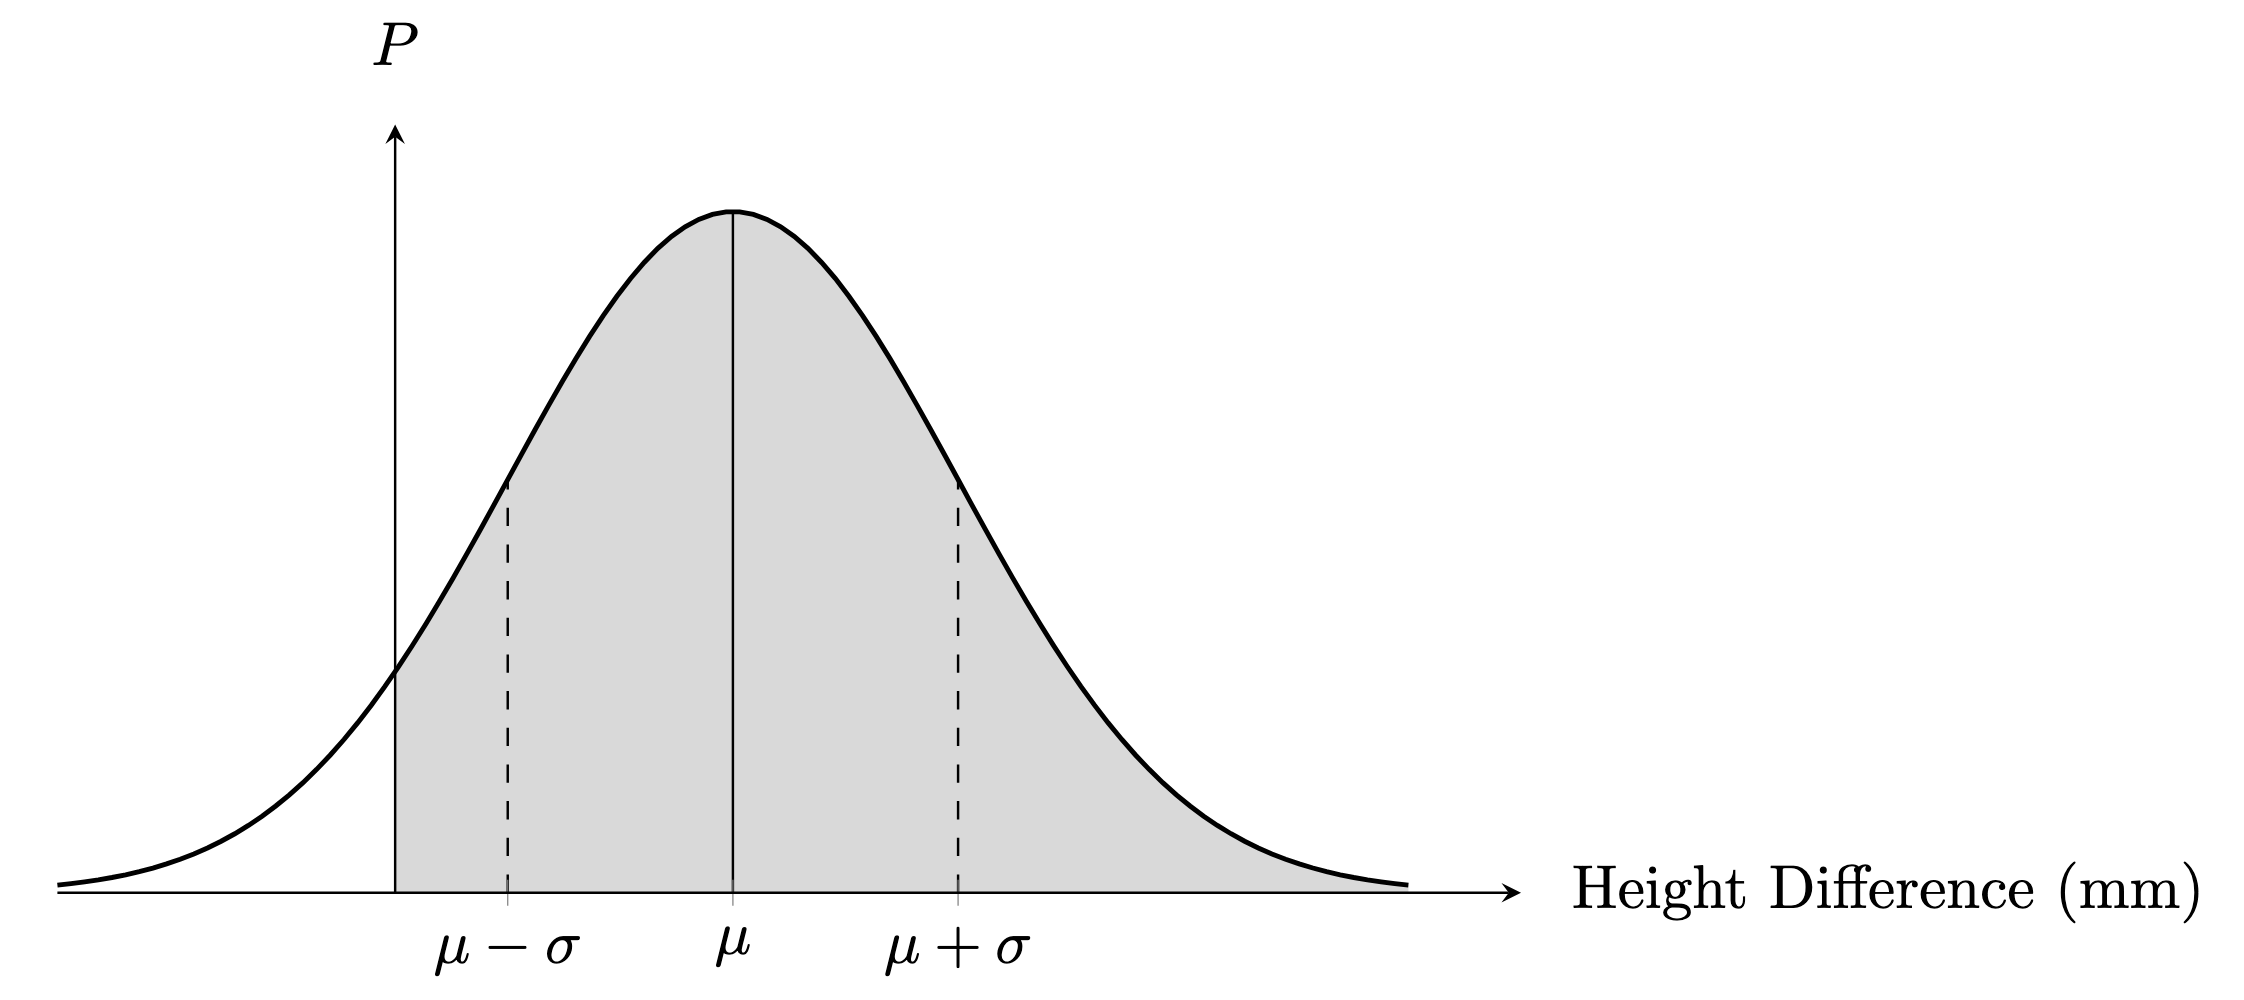
\includegraphics[width=0.75\linewidth]{height-distribution}
    \caption{Distribution of the difference in heights, with $P(\text{height difference} > 0)$ shaded.}
    \label{fig:height_diff_shaded}
\end{figure}

\subsection{Part 2:}\label{subsec:part-2:}
Now that the first part to our overarching question has been answered, we will assess whether this trend depends on cultural factors.
To do this, it is now necessary to more directly relate both the Galton and Marsh datasets.
Therefore, our new null hypothesis is $H_0:p_1=p_2$ while the alternative hypothesis is that $H_a:p_1 \neq p_2$ (if a one-tail test were being performed, $p_1>p_2$ or $p_1<p_2$).
To determine whether there is a notable difference between the proportions, we introduce the following statistic analogous to the previous one:

\begin{equation}
    z=\frac{\hat{p_1}-\hat{p_2}-(p_1-p_2)}{\sqrt{\frac{\overline{p}(1-\overline{p})}{n_1}+\frac{\overline{p}(1-\overline{p})}{n_2}}} 
    \label{eq:taller-male-proportion-z-statistic}
\end{equation}
where $\bar{p}=\frac{x_1+x_2}{n_1+n_2}$ is the average proportion and $x_1$ is the number of couples with the male being taller out of the $n_1$ couples in the first data set.
It is interesting that in both data sets, 188 couples satisfy the condition that the husband is taller; this does translate to different actual proportions, though, because the sample sizes are different.
In maintaining consistency, the Marsh data is assigned as \#1 and the Galton as
\#2. Using $\hat{p}_i$ as the actual proportion for data set $i$, we determine that $z=1.0940$.
This value is cleanly within a confidence interval of 95\% ($z \in [-1.96, 1.96]$ as before), which means that we fail to reject the null hypothesis.
There is, therefore, not a statistically significant difference in the proportion of couples with a taller male between the two datasets.
This finding is strong evidence that couples across different populations tend to have a taller male.

This evidence strongly suggests that the proportion of couples with a taller male is the same across datasets of different time periods
To strengthen the argument, we must confirm whether this result is due to our datasets covering populations which are too similar.
To study the average heights for each set, we introduce here the student-t distribution, which approaches the normal distribution as the sample size increases ($n\rightarrow{\infty}$). The actual expression is given by the following:
\begin{equation}
P(X<t)=\frac{1}{B(\frac{1}{2},\frac{\nu}{2})\sqrt{\nu}}\int_{-\infty}^t(1+\frac{x^2}{\nu})^{-(\nu+1)/2}dx
\label{eq:t-score-integral}
\end{equation}
where $B(x,y)=\int_0^1 t^{x-1}(1-t)^{y-1}dt$ is the Beta function and $\nu$ is the degrees of freedom.
What are degrees of freedom?
Well, it is basically the number of values that are allowed to vary; take for the sake of illustration, a class of ten students.
If you know the class average on an exam and in addition know the individual scores of nine students, it is quite straightforward to find the score of the last student.
One must simply multiply the mean by the sample size and subtract the individual scores.
More generally, there would be $n-1$ degrees of freedom for $n$ students.
Going back to our pertaining discussion, the student-t (no pun intended) distribution, as beautiful as it seems, can be quite complex to work with in this introductory paper, so the following simpler test statistic expression will be utilized:
\begin{equation}
t=\frac{\bar{x}_1-\bar{x}_2-(\mu_1-\mu_2)}{\sqrt{\frac{s_1^2}{n_1}+\frac{s_2^2}{n_2}}}
\label{eq:comparing-heights-by-sex-across-datasets-t-test}
\end{equation}
with the approximation that $\nu=\min\{n_1-1,n_2-1\}$ and positing the null hypothesis as $\mu_1=\mu_2$.
For the passionate reader, the actual degrees of freedom for non-equal variances is
\begin{equation}
\nu=\frac{(A+B)^2}{\frac{A^2}{n_1-1}+\frac{B^2}{n_2-1}}
\label{eq:degrees-of-freedom-for-nonequal-variances}
\end{equation}
where $A=\frac{s_1^2}{n_1}$ and $B=\frac{s_2^2}{n_2}$.
Furthermore, if the variances were actually known to be equal (which would be the case if both samples came from the same population), then $\nu=n_1+n_2-2$ while the $s_1$ and $s_2$ in \eqref{eq:t-score-integral} would be replaced with the pooled sample variance:
\begin{equation}
    s_p^2\coloneqq\frac{(n_1-1)s_1^2+(n_2-1)s_2^2}{(n_1-1)+(n_2-1)}.
    \label{eq:pooled-sample-variance}
\end{equation}

Attempting once more to focus on the present endeavor, we observe that $\nu=198$ and according to Equation \eqref{eq:comparing-heights-by-sex-across-datasets-t-test}, $t_{males}=-4.1573$ and $t_{females}=-3.9111$ whose magnitudes are greater than 1.97 (which one can find by solving \eqref{eq:t-score-integral} with $t=0.95$).
These large t-scores indicate that the groups are significantly different and the null hypothesis must be rejected.
This conclusion is also supported by the p-score for men and women being very close to zero (if the probability for the t-score is less than 0.5, the null hypothesis is rejected).
This finding supports the robustness our earlier conclusion that the tendency for the male in a couple to be taller exists across different populations.

Earlier in this paper we used the test statistic in \eqref{eq:taller-male-proportion-z-statistic} to determine whether there was a statistically significant difference between the two datasets in the proportion of couples who had a taller man.
With our last major test, we will test a similar hypothesis, but one that focuses not on the number of couples with a taller male, but on the magnitude of the height difference.
We will use the following $t$-statistic:
\begin{equation}
   t=\frac{\bar{d}-\mu_d}{\bar{s}/\sqrt{n}}
   \label{eq:difference-t-test}
\end{equation}
where $\bar{d}$ is the mean of the differences in heights and $\bar{s}$ is the standard deviation in the difference in heights.
$\mu_d$ is the theoretical mean that we test against.
Our null hypothesis is $H_0: \bar{d} = 0$, and our alternative hypothesis is $H_a:\bar{d} \ne 0$.
We want to know if $\bar{d}$ is above the critical $t$-score for 95\% confidence ($t\approx1.65$ for both datasets), so this is a one-tailed test.
Since, in this case, we are comparing $\bar{d}$ to 0, we set $\mu_d=0$.
Using \eqref{eq:difference-t-test}, we find that $t_{Marsh}=24.8399$ and $t_{Galton}=22.6810$.
Since both of these are much greater than 1.65, we must reject the null hypothesis for both datasets.
From this result we can conclude that the magnitude of the height difference between males and females is both positive (i.e.\ the man is taller) and statistically significant.

Let us test one final hypothesis: there is no difference between the mean height difference of both datasets ($H_0:\bar{d}_1\neq \bar{d}_2$).
We will use a two-tailed $t$-test at a 95\% confidence level to test this claim.
The $t$-statistic for this hypothesis can be calculated using an equation analogous to \eqref{eq:comparing-heights-by-sex-across-datasets-t-test}, but which replaces $\bar{x}_i$ with $\bar{d}_i$.
Plugging the calculated statistics from the two datasets into the equation described, we find that $t=-0.5588$.
This falls neatly within a 95\% confidence interval ($t\in[-1.97,1.97]$ for $\nu=\min\{n_1-1, n_2-1\}=198$ like before), so we fail to reject the null hypothesis.
From this result we can conclude that there is not a significant difference between the mean height difference of the two datasets.

\section{Conclusion}\label{sec:conclusion}
To summarize our findings:

\begin{itemize}
    \item In both datasets, the mean height of men is greater than the mean height of women.
    \item People in the Marsh dataset were shorter on average than those in the Galton dataset.
    \item There is a slight positive correlation between spouse heights, but this correlation is too small to have any predictive power.
    \item The difference in the heights of men and women can be accurately predicted using a bivariate normal distribution.
    \item We failed to reject the null hypothesis that the actual proportion of taller-male couples is equal to the proportion expected from the model.
    \item The height difference between men and women is statistically significant.
    \item There is not a statistically significant difference in the proportion of taller-male couples between the two datasets.
    \item There is not a statistically significant difference between the average height gap of the two time periods.
\end{itemize}

From these findings, it is certainly the case that men tend to marry women that are shorter than them.
However, the dataset provides no evidence that this tendency is the result of men preferring to marry shorter women or women preferring to marry taller men.
It is simply the case that men tend to be taller than women, on average.
Such a preference may exist, but proving its existence would require qualitative methods.
We also showed that the two datasets describe significantly different populations.
While this lends credence to the idea that we have discovered a general trend, we would need more data from different time periods and cultures to strengthen the evidence for this conclusion.

This paper has hopefully showcased the intricacies of statistics and its probabilistic repercussions on human understanding of large-scale phenomena.
We have demonstrated how this field can attempt to find answers to curious questions many might have deemed unknowable in the past.
Yet, through its innate limitations and assumptions, statistics fosters a greater level of transparency and humility among the scientific community which holds promise for advancing many analytical fields of study for the benefit of mankind.

\section{Appendix}\label{sec:appendix}

The mean, standard deviation, and correlation statistics were calculated using the built-in dataframe methods provided by the Pandas library \parencite{pandas}.
For hypothesis testing, $p$-values and critical values were derived from the Standard Normal ($Z$) and student-$t$ distributions using the stats module from the Scipy library \parencite{scipy}.
In particular, the survival function (sf) was employed for right-tail probability calculations, and the percent-point function (ppf) was used to determine critical thresholds for significance.
The code used to calculate the results in this paper is hosted at the following GitHub repository: \url{https://github.com/jkqq-0/prob-and-stat-project-2}.

\printbibliography

\end{document}
